\chapter{Design of the control system} \label{ch4}

In the previous chapters, we outlined deep reinforcement learning fundamentals and the most critical underlying concepts, and then we discussed the choice made about the technologies to use as baselines for our experiments. The decision fell on Anki Cozmo because of the high-quality SDK provided to developers and the versatility and flexibility provided by PyTorch, especially in a research context.

The next step in this thesis is the merge of reinforcement learning theory with the tool presented previously. Indeed, this chapter aims to describe this merge process that results in the design of the control system for reinforcement learning experiments with Anki Cozmo. The work presented in this section represents one of the contributions of our thesis and the necessary step to start reinforcement learning experiments.

The primary source of inspiration to develop this control system came from \cite{kendall2018learning,kendall2019learning}. As the authors suggest, this publication represents the first reinforcement learning self-driving experiment where a car learned to drive by trial and error. They first trained the model using a simulator and then managed to transfer the learning in real-world experiments. The authors implemented a system where the car was able to drive by itself after few episodes, with the aid of the human in the driving seat in the learning process: he stops the car when it is going to run off the road or in a dangerous situation and must reposition it to start the next learning episode.
The human-robot interaction is crucial in this type of experiment because it is the source of all improvements and flaws of the learning results: the robot learns which actions are worthy and which are not, but the human is the one who decides the correctness of each action, carrying its unconscious bias in the algorithm. We will discuss the experiments and their results intensely in \vref{ch5,ch6}.

The outline of the whole ecosystem with the description of interfaces, frameworks and technologies used occupies the first section of the chapter. This part also comprehends a discussion about DDPG \cite{lillicrap2015continuous} and SAC \cite{haarnoja2018soft, haarnoja2018alg} implementation with references to the choice made in terms of hyper-parameters and problems faced.

The second part of the chapter aims to describe the implementation of Anki Cozmo OpenAI Gym environment from the problem formalisation as MDP to the implementation of human-robot interaction.

In the final section of this chapter, the design and setup of the real track will be discussed together with a discussion about the problems faced and the choice made to overcome them.



\tikzset{every picture/.style={line width=0.75pt}} %set default line width to 0.75pt        

\begin{figure}
	\tikzset{every picture/.style={line width=0.75pt}} %set default line width to 0.75pt    
	\centering    
	\scalebox{0.85}{
\begin{tikzpicture}[x=0.75pt,y=0.75pt,yscale=-1,xscale=1]
%uncomment if require: \path (0,438); %set diagram left start at 0, and has height of 438

%Image [id:dp06991158821872456] 
\draw (239.75,55) node  {
\includegraphics[width=115.13pt,height=52.5pt]{img/python.png}};
%Image [id:dp3729269645681633] 
\draw (240.25,200.5) node  {
\includegraphics[width=46.88pt,height=50.25pt]{img/gym.png}};
%Image [id:dp09149607927009118] 
\draw (94.75,200.91) node  {
\includegraphics[width=124.13pt,height=25.37pt]{img/pytorch.png}};
%Image [id:dp30806594376010465] 
\draw (370.92,200) node  {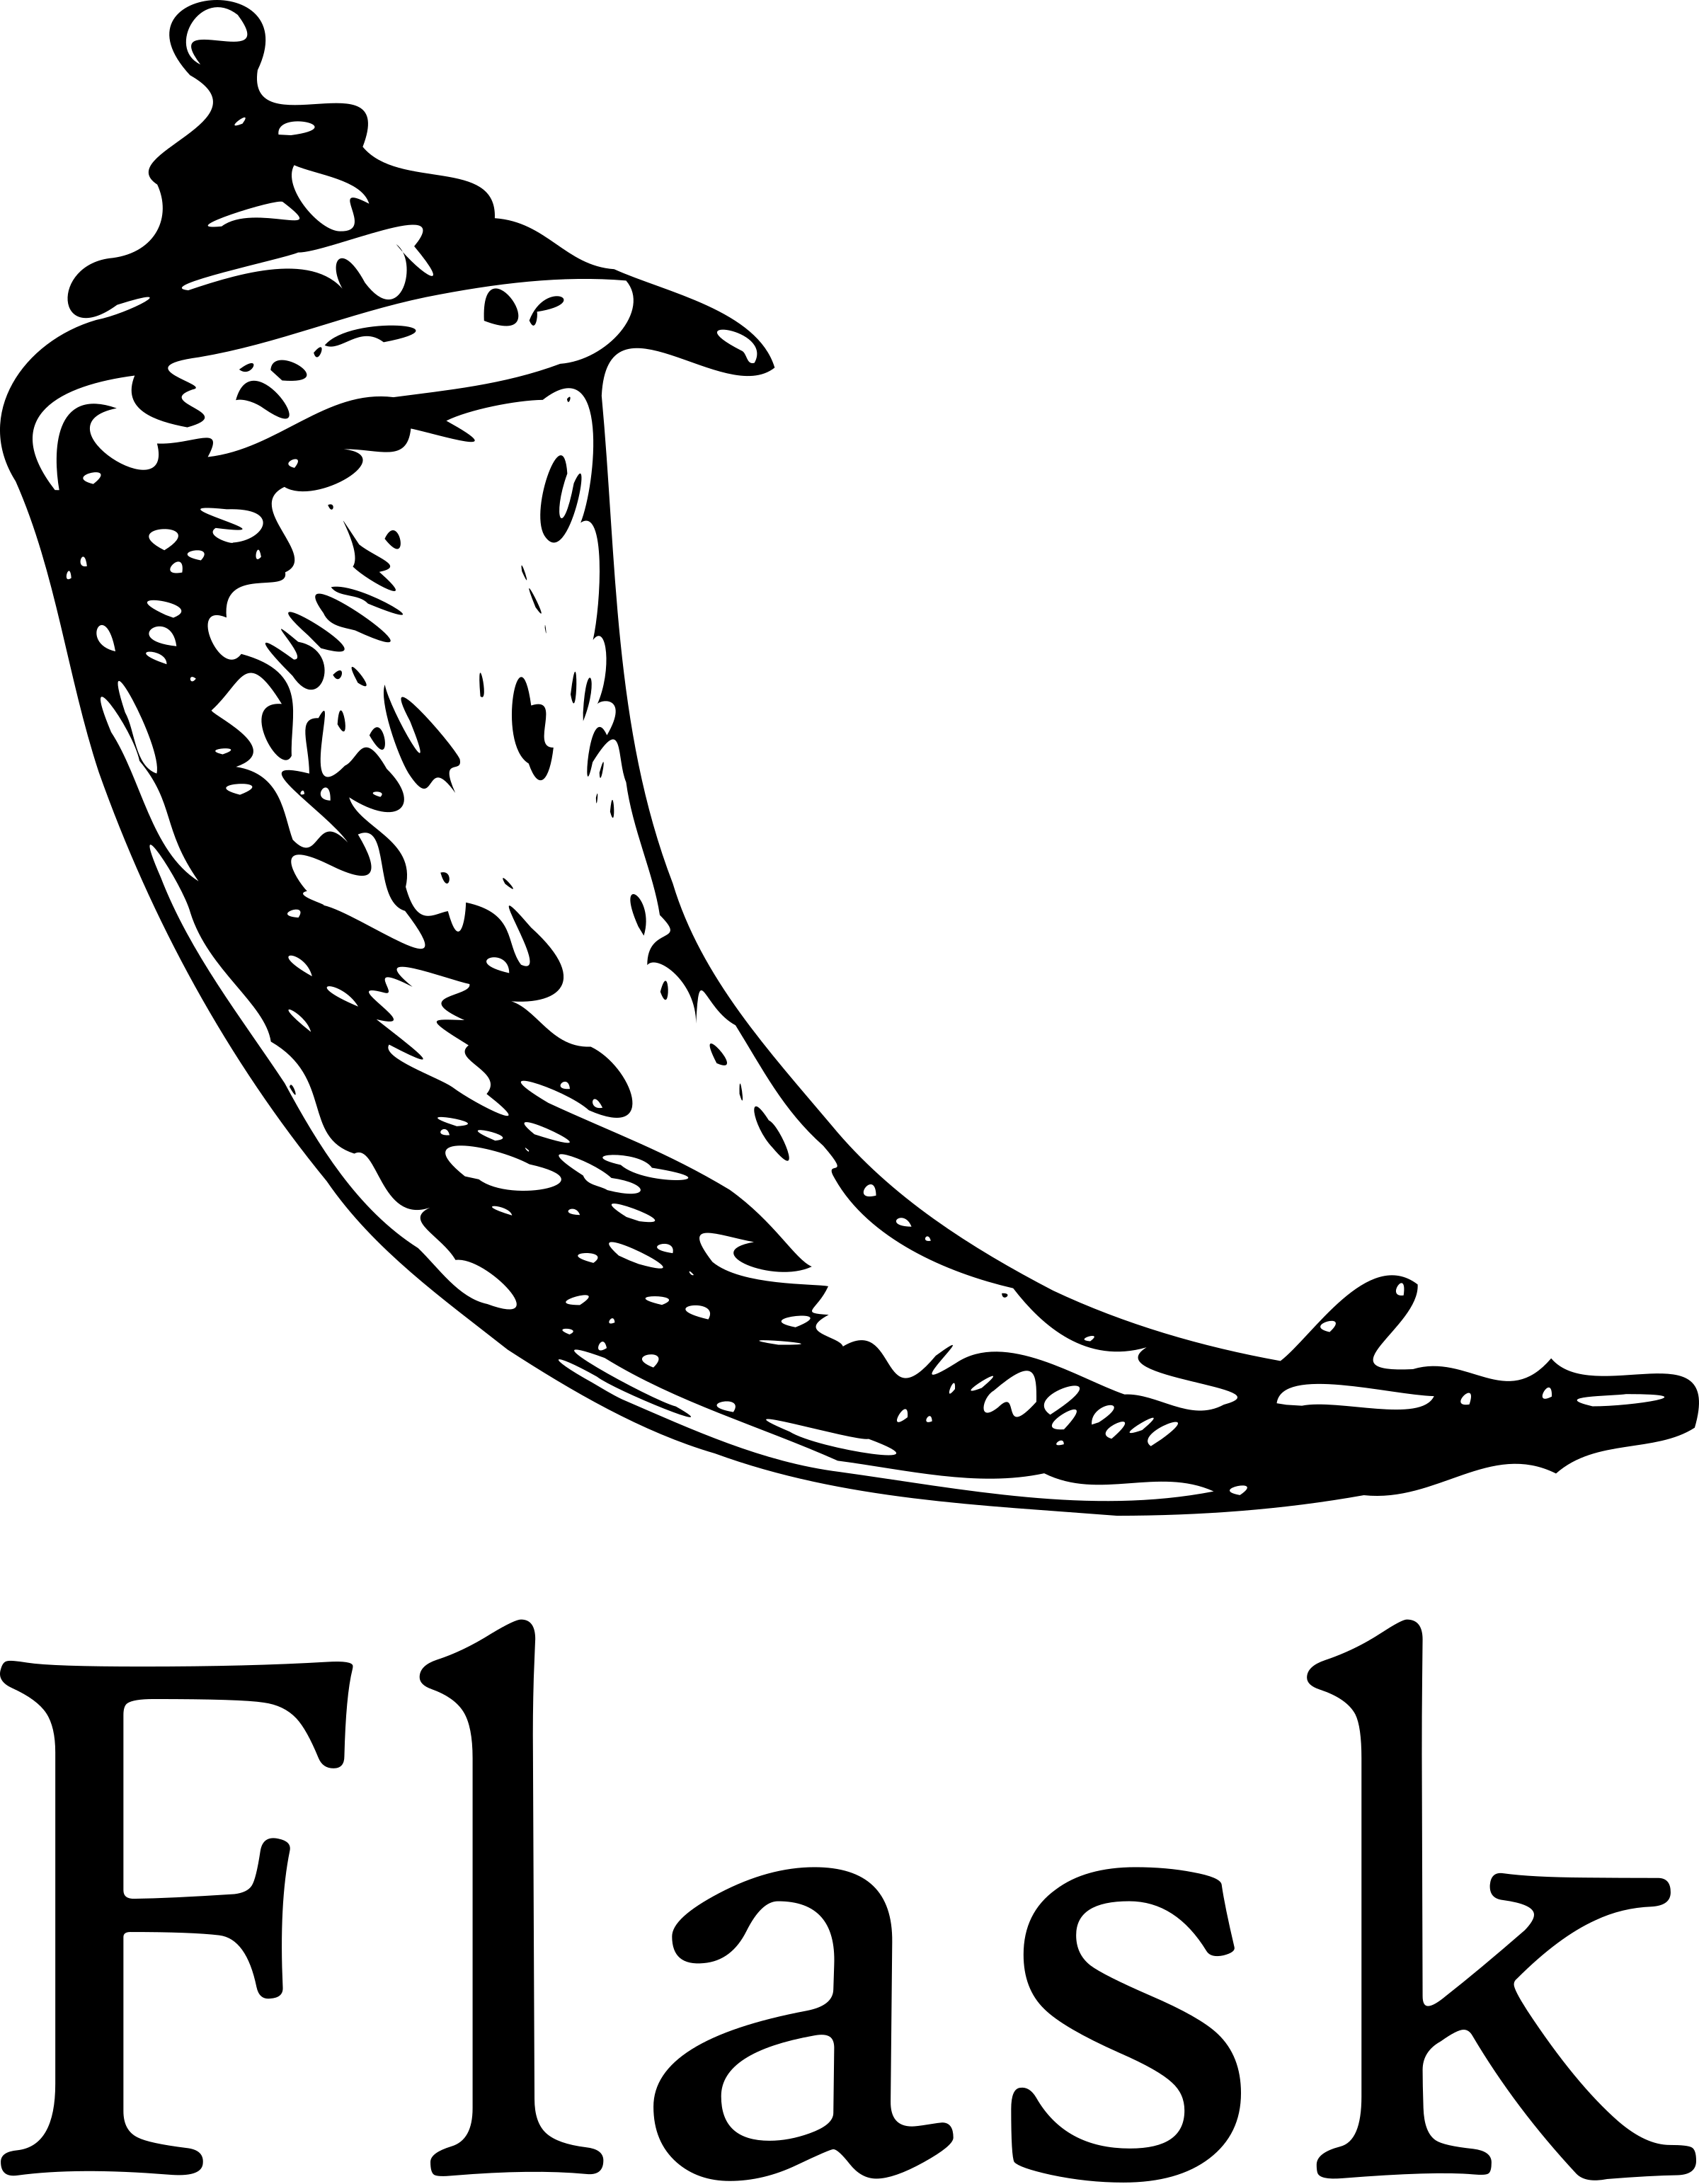
\includegraphics[width=40.38pt,height=52.5pt]{img/flask.png}};
%Straight Lines [id:da3933293266418665] 
\draw    (239.98,93) -- (239.52,159) ;
\draw [shift={(239.5,162)}, rotate = 270.4] [fill={rgb, 255:red, 0; green, 0; blue, 0 }  ][line width=0.08]  [draw opacity=0] (8.93,-4.29) -- (0,0) -- (8.93,4.29) -- cycle    ;
\draw [shift={(240,90)}, rotate = 90.4] [fill={rgb, 255:red, 0; green, 0; blue, 0 }  ][line width=0.08]  [draw opacity=0] (8.93,-4.29) -- (0,0) -- (8.93,4.29) -- cycle    ;
%Straight Lines [id:da24057878811893751] 
\draw    (167.75,200.25) -- (203.75,200.25) ;
\draw [shift={(206.75,200.25)}, rotate = 180] [fill={rgb, 255:red, 0; green, 0; blue, 0 }  ][line width=0.08]  [draw opacity=0] (8.93,-4.29) -- (0,0) -- (8.93,4.29) -- cycle    ;
\draw [shift={(164.75,200.25)}, rotate = 0] [fill={rgb, 255:red, 0; green, 0; blue, 0 }  ][line width=0.08]  [draw opacity=0] (8.93,-4.29) -- (0,0) -- (8.93,4.29) -- cycle    ;
%Straight Lines [id:da10061083103025648] 
\draw    (283.75,199.58) -- (334.5,199.58) ;
\draw [shift={(337.5,199.58)}, rotate = 180] [fill={rgb, 255:red, 0; green, 0; blue, 0 }  ][line width=0.08]  [draw opacity=0] (8.93,-4.29) -- (0,0) -- (8.93,4.29) -- cycle    ;
\draw [shift={(280.75,199.58)}, rotate = 0] [fill={rgb, 255:red, 0; green, 0; blue, 0 }  ][line width=0.08]  [draw opacity=0] (8.93,-4.29) -- (0,0) -- (8.93,4.29) -- cycle    ;
%Image [id:dp8556439958741602] 
\draw (558,186) node  {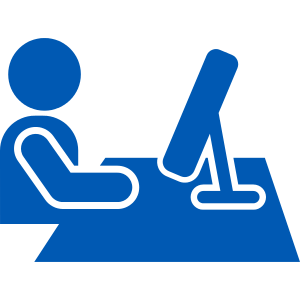
\includegraphics[width=52.5pt,height=52.5pt]{img/user.png}};
%Straight Lines [id:da26821981951432505] 
\draw    (407.75,184.58) -- (479.67,184.58) ;
\draw [shift={(482.67,184.58)}, rotate = 180] [fill={rgb, 255:red, 0; green, 0; blue, 0 }  ][line width=0.08]  [draw opacity=0] (8.93,-4.29) -- (0,0) -- (8.93,4.29) -- cycle    ;

%Straight Lines [id:da7643998387312995] 
\draw    (408.75,214.58) -- (480.67,214.58) ;

\draw [shift={(405.75,214.58)}, rotate = 0] [fill={rgb, 255:red, 0; green, 0; blue, 0 }  ][line width=0.08]  [draw opacity=0] (8.93,-4.29) -- (0,0) -- (8.93,4.29) -- cycle    ;
%Straight Lines [id:da5051570254396728] 
\draw    (240.05,244) -- (240.45,268) ;
\draw [shift={(240.5,271)}, rotate = 269.05] [fill={rgb, 255:red, 0; green, 0; blue, 0 }  ][line width=0.08]  [draw opacity=0] (8.93,-4.29) -- (0,0) -- (8.93,4.29) -- cycle    ;
\draw [shift={(240,241)}, rotate = 89.05] [fill={rgb, 255:red, 0; green, 0; blue, 0 }  ][line width=0.08]  [draw opacity=0] (8.93,-4.29) -- (0,0) -- (8.93,4.29) -- cycle    ;
%Rounded Rect [id:dp9694318857670313] 
\draw   (2,69.4) .. controls (2,34.94) and (29.94,7) .. (64.4,7) -- (588.1,7) .. controls (622.56,7) and (650.5,34.94) .. (650.5,69.4) -- (650.5,256.6) .. controls (650.5,291.06) and (622.56,319) .. (588.1,319) -- (64.4,319) .. controls (29.94,319) and (2,291.06) .. (2,256.6) -- cycle ;
%Image [id:dp9562999520117128] 
\draw (99,377) node  {
\includegraphics[width=52.5pt,height=52.5pt]{img/tablet.png}};
%Straight Lines [id:da22030012036466173] 
\draw    (95.5,290) -- (186.5,290) ;
\draw [shift={(189.5,290)}, rotate = 180] [fill={rgb, 255:red, 0; green, 0; blue, 0 }  ][line width=0.08]  [draw opacity=0] (8.93,-4.29) -- (0,0) -- (8.93,4.29) -- cycle    ;

%Straight Lines [id:da28839463654139263] 
\draw    (95.5,290) -- (95.5,334) ;
\draw [shift={(95.5,337)}, rotate = 270] [fill={rgb, 255:red, 0; green, 0; blue, 0 }  ][line width=0.08]  [draw opacity=0] (8.93,-4.29) -- (0,0) -- (8.93,4.29) -- cycle    ;

%Straight Lines [id:da2120925552884272] 
\draw  [dash pattern={on 0.84pt off 2.51pt}]  (154.75,380.58) -- (470.5,380.58) ;
\draw [shift={(473.5,380.58)}, rotate = 180] [fill={rgb, 255:red, 0; green, 0; blue, 0 }  ][line width=0.08]  [draw opacity=0] (8.93,-4.29) -- (0,0) -- (8.93,4.29) -- cycle    ;
\draw [shift={(151.75,380.58)}, rotate = 0] [fill={rgb, 255:red, 0; green, 0; blue, 0 }  ][line width=0.08]  [draw opacity=0] (8.93,-4.29) -- (0,0) -- (8.93,4.29) -- cycle    ;
%Image [id:dp7151280650926004] 
\draw (533.32,370) node  {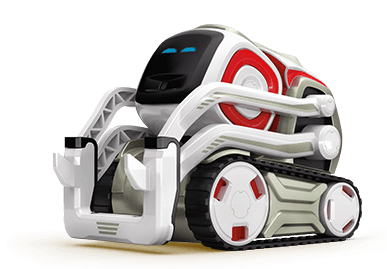
\includegraphics[width=81.48pt,height=58.5pt]{img/cozmo.png}};

% Text Node
\draw (556,230) node   [align=left] {Human-Robot Interaction};
% Text Node
\draw (445,174) node  [font=\footnotesize] [align=left] {Image};
% Text Node
\draw (447,202) node  [font=\footnotesize] [align=left] {Commands};
% Text Node
\draw (501,24) node   [align=left] {\textbf{Development Machine}};
% Text Node
\draw    (196.5,274.5) -- (287.5,274.5) -- (287.5,299.5) -- (196.5,299.5) -- cycle  ;
\draw (242,287) node   [align=left] {Cozmo SDK};
% Text Node
\draw (100,423) node   [align=left] {\textbf{Android Device}};
% Text Node
\draw (120,276) node   [align=left] {{\footnotesize ADB}};
% Text Node
\draw (235,367) node   [align=left] {Wi-Fi Connection};
% Text Node
\draw (536,420) node   [align=left] {\textbf{Cozmo}};


\end{tikzpicture}
}
	\caption[Interaction Robot/Application]{Interaction between the Robot and the mobile application stack. The robot main program interacts with the Cozmo Engine (C++) implemented in the mobile application through a proprietary TCP protocol established using and ad-hoc WiFi connection. \cite{mellon2017cognitive}}
	\label{fig:cozmotear1}
\end{figure}


% \todomacaluso{
% 	\begin{itemize}
% 		\item Introduction to the chapter
% 		\item General description of the control systems with a diagram representing all the technologies involved.
% 		\item Setup of the algorithms (DDPG, SAC)
% 		      \begin{itemize}
% 			      \item We decided to rewrite both algorithms without using libraries directly. The first motivation was didactical, implementing from scratch is helpful to understand the practical implementation of the algorithm better, but also to make it possible to implement the singularity of the real Cozmo environment.
% 			      \item The interaction with OpenAI Gym and PyTorch
% 			      \item Discussion about Hyper-Parameters and the problems faced in the real world situation in the selection of these parameters.
% 		      \end{itemize}
% 		\item Setup and implementation of CozmoEnv
% 		      \begin{itemize}
% 			      \item Technologies used to implement the interaction between the Cozmo SDK and OpenAI Gym.
% 			      \item Differences from the simulated environment caused by the need for direct human interaction.
% 			      \item Implementation of human interaction in the system.
% 		      \end{itemize}
% 		\item Setup of the real Environment
% 		      \begin{itemize}
% 			      \item The Track design
% 			      \item Analysis of the problems:
% 			            \begin{itemize}
% 				            \item Reflection
% 				            \item Background and Horizon
% 			            \end{itemize}
% 			      \item (Single Line Track)
% 		      \end{itemize}
% 	\end{itemize}
% }

% \section{The track}

% The design and training of a good driving model cannot go beyond the construction and design of the road. For this reason, some time was spent searching the better way to build a path where to train Cozmo.
% This section aims to present the central concept and decisions made about the design of the track for the experiments, starting from the materials used, up to the description of the dimensional choices applied.

% \subsection{Track requirements}

% It is essential to explain the primary needs of the road before proceeding with the description of the choices made.

% Firstly, the track needs to be easily transportable to allow various attempt with different locations and environmental conditions that could affect the training phase. In particular, it is necessary to use a material less reflective as possible to avoid problems during the learning process.
% Another crucial factor is the dimension of the lane, which must reproduce an environment similar to the real one. It can be done analyzing the ratio of the size of a vehicle to the width of a road. On average, a family car is about $160$-$170$cm large, while a lane width can vary between $275$cm and $375$cm. Cozmo width is about $5.5$cm, which results in a ratio of $1/30$. Therefore, the scaled lane must be between $9$cm and $12.5$cm.

% \subsection{Track design and materials}

% The first choice to make is the one about the type of material to use as terrain for the track. The first choice was the black floor of the Data Science laboratory of Eurecom. It was useful only during the initial design and development of the control system to build small pieces of track in which testing functionalities. This solution had numerous drawbacks such as the impracticality to transport and high light reflection. 

% The following list provides a brief report of the various solutions taken into account during the thesis, together with an analysis of advantages and drawbacks.

% \begin{itemize}
% 	\item \textit{Covering fabric}: this material is easily transportable, but it has a high light reflection, and its structure is prone to make wrinkles and dunes challenging to remove.
% 	\item \textit{Tar paper}: this solution slightly diminished the reflection problem compared to the previous choice, but the material was fragile and with the same drawbacks of the covering fabric.
% 	\item \textit{Cotton fabric}: this solution offers an easily  transportable material with reduced light reflection where it is easy to remove wrinkles and dunes.
% \end{itemize}

% Summing up, it is noticeable from this analysis that the cotton fabric provides the right trade-off among all requirements reported before.

% The structure of the road is also composed by the lane. The implementation of this part was done using a simple paper tape of width equal to $2.5$cm. As described in the beginning of this section, the width of the lane must be between $9$cm and $12.5$cm to provide a context similar to the real one. Because of the narrow and limited angle of vision provided by Cozmo camera, $10$cm-width was set: positioning the tape with a distance greater than $10$cm would result in a great part of the tape outside the view of the camera.